\section{Tulokset}

Kuvassa \ref{fig:music} on simuloitu MUSIC-algoritmia sekä kiinteällä että vapaalla orientaatiolla. Simuloinneissa kolme lähdedipolia sijoitettiin aivokuorelle, jotka on merkitty punaisina ympyröinä ja topografia on muodostettu MUSIC-algoritmin paikannusfunktion arvoista.

Kuvissa \ref{fig:RAPfix} ja \ref{fig:RAPfree} on simuloitu RAP-MUSIC- algoritmia kiinteällä ja vapaalla orientaatiolla. Kuvissa musta rasti kuvaa paikannusfunktion maksimiarvon paikkaa ja löydetyt dipolit merkataan punaisella neliöllä. Vastaavasti kuvissa \ref{fig:TRAPfix} ja \ref{fig:TRAPfree} on kuvattu TRAP-MUSIC:n käyttöä kiinteällä ja vapaalla orientaatiolla. 

Kuvista huomataan, että MUSIC vapaalla orientaatiolla saa aikaan suurempia aktiivisuuden alueita kuin kiinteällä orientaatiolla, mikä vaikeuttaa lähteiden tarkkaa paikantamista. 

Tavallisen MUSIC-algoritmin yksi ongelmista on oikeiden lähteiden erottaminen vääristä \citep{Mosher1998RecursiveLocalization}. Oikeiden lähteiden löytäminen kuvasta voi olla vaikeaa, kun lähteiden määrä on suuri. Lisäksi MUSIC-algoritmilla on vaikeuksia löytää synkronoituja lähteitä \citep{Mosher1999SourceMUSIC}. Kaikilla MUSIC-algoritmin versioilla on vaikeuksia löytää hyvin lähellä toisiaan olevia dipoleita. RAP- ja TRAP-MUSIC:ssa löydettyä lähdettä projisoidessa pois häviää myös löytämättä jääneen lähteen topografiaa, jolloin viereistä lähdettä ei välttämättä löydetä.


\begin{figure}[hb]
    \begin{minipage}{0.5\textwidth}
        \centering
        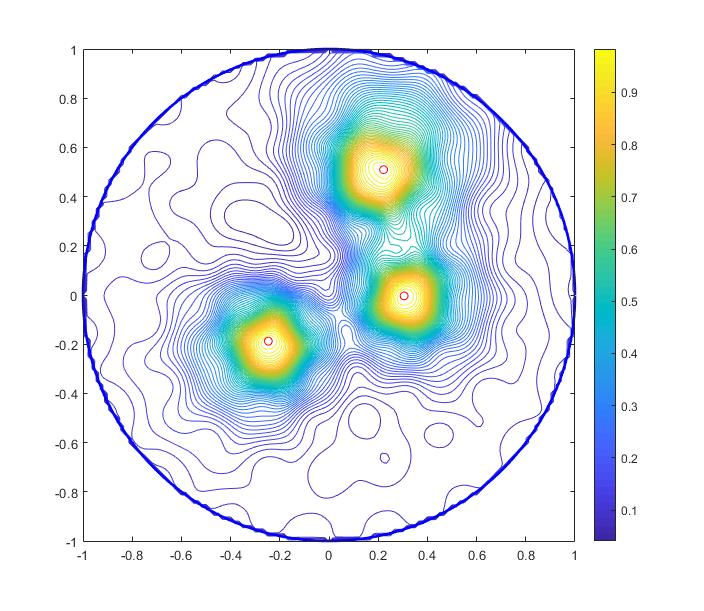
\includegraphics[width=\textwidth]{mfix.jpg} 
    \end{minipage}
    \begin{minipage}{0.5\textwidth}
        \centering
        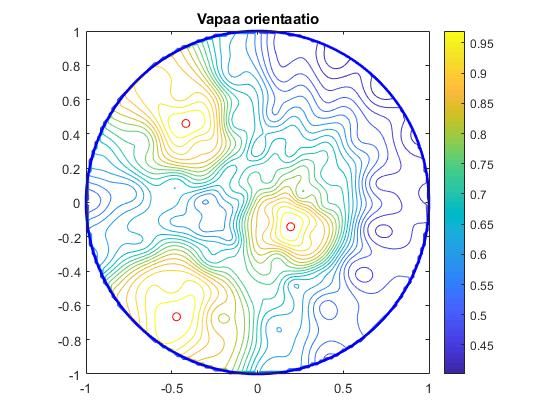
\includegraphics[width=\textwidth]{mfree.jpg}
    \end{minipage}
    \caption{MUSIC-algoritmilla piirretyt topografiakuvat kiinteän ja vapaan orientaation MUSIC-algoritmeilla simuloidulla datalla. Punaiset ympyrät kuvaavat sijoitettuja lähteitä.}
    \label{fig:music}
\end{figure}

\clearpage

\begin{figure}
    \centering
    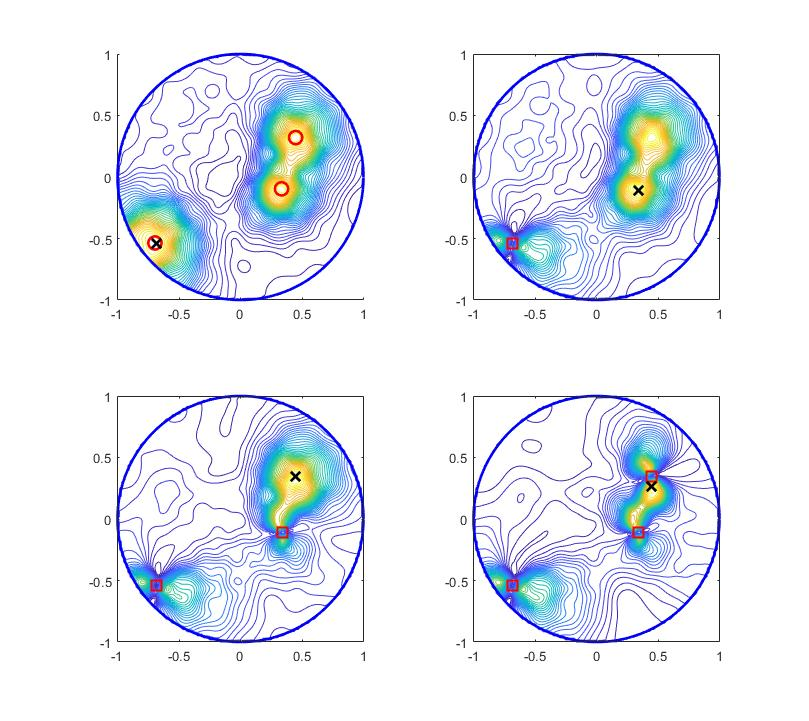
\includegraphics[width=\textwidth]{RAPfixed.jpg}
    \caption{RAP-MUSIC kiinteällä orientaatiolla. Musta rasti kuvaa iteraatiokierroksen paikannusfunktion maksimia ja punaiset ympyrät löydettyjä lähteitä.}
    \label{fig:RAPfix}
\end{figure}

\clearpage
\begin{figure}
    \centering
    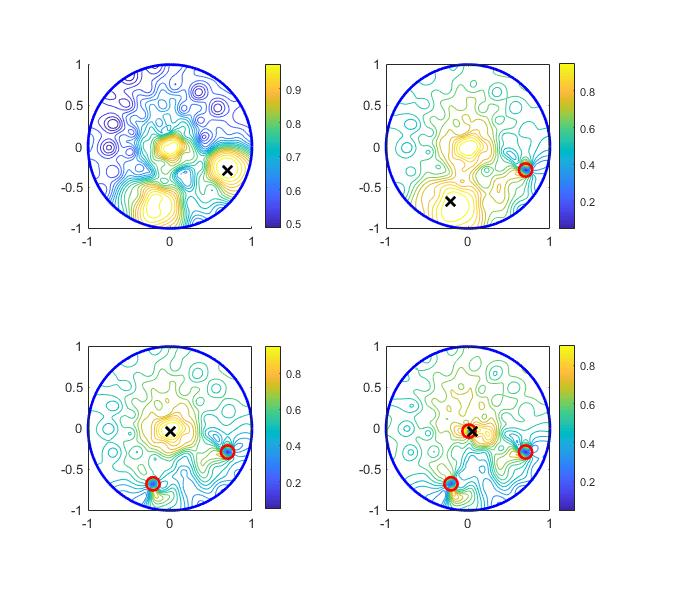
\includegraphics[width=\textwidth]{RAPfree.jpg}
    \caption{RAP-MUSIC vapaalla orientaatiolla. Merkinnät ovat samat kuin kuvassa \ref{fig:RAPfix}.}
    \label{fig:RAPfree}
\end{figure}

\clearpage
\begin{figure}[ht]
    \centering
    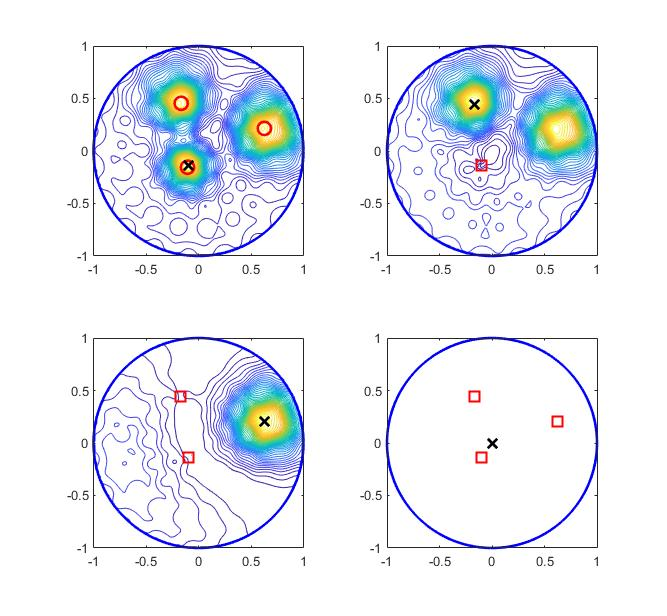
\includegraphics[width = 0.65\textwidth]{trap.jpg}
    \caption{TRAP-MUSIC kiinteällä orientaatiolla}
    \label{fig:TRAPfix}
\end{figure}

\begin{figure}[h!]
    \centering
    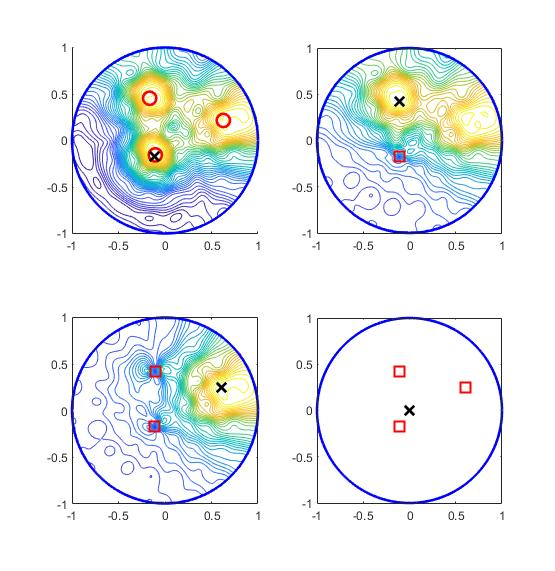
\includegraphics[width = 0.65\textwidth]{trapp.jpg} 
    \caption{TRAP-MUSIC vapaalla orientaatiolla}
    \label{fig:TRAPfree}
\end{figure}

\clearpage
\begin{figure}[h]
    \begin{minipage}{0.5\textwidth}
        \centering
        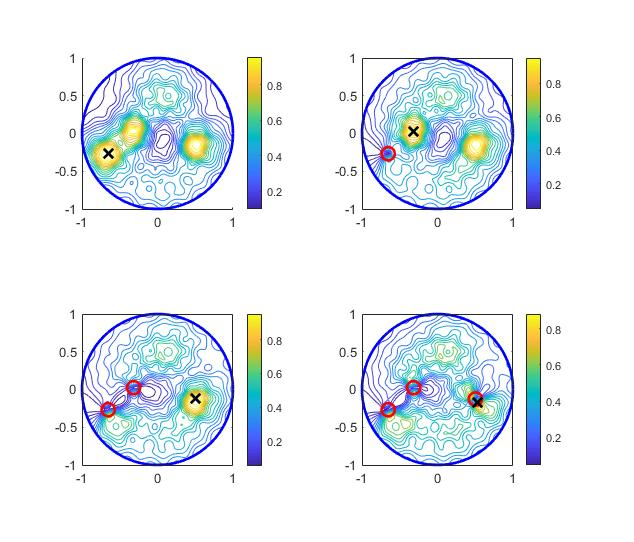
\includegraphics[width=\textwidth]{RAPvsTRAP2.jpg}
    \end{minipage}
    \begin{minipage}{0.5\textwidth}
        \centering
        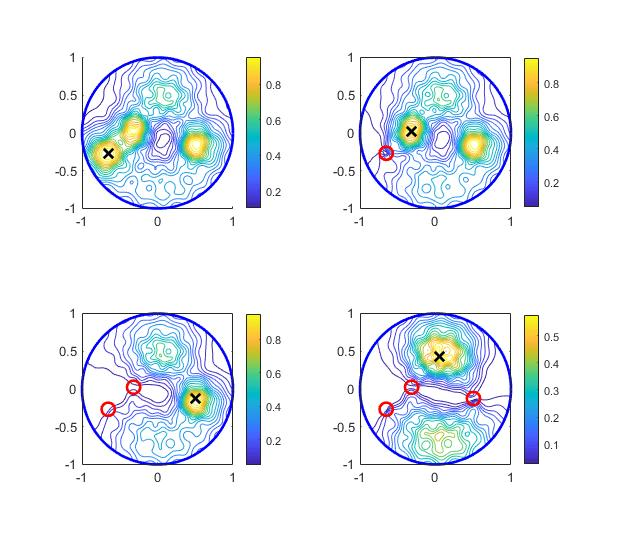
\includegraphics[width=\textwidth]{RAPvsTRAP1.jpg}
    \end{minipage}
    \caption{RAP- ja TRAP-MUSIC:n vertailua. Kuvista voi huomata, kuinka paljon paremmin TRAP-MUSIC poistaa topografiaa löydettyjen lähteiden ympäriltä.}
    \label{fig:rapvstrap}
\end{figure}

\begin{figure}
    \centering
    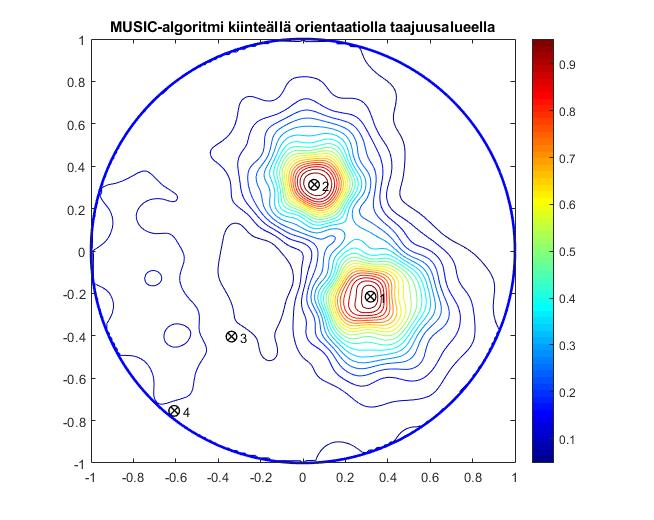
\includegraphics[width=\textwidth]{fMUSIC.jpg}
    \caption{Esimerkki MUSIC-algoritmin käytöstä taajuusalueella. Simuloidusta datasta haettiin 12 Hz taajuudella olevia lähteitä. Sijoitetut lähteet merkittiin mustilla ruksatuilla ympyröillä ja numeroitiin. Lähteitä oli yhteensä neljä, joista kaksi oli 12 Hz taajuudella eli numerot 1 ja 2.}
    \label{fig:fMUSIC}
\end{figure}

\clearpage
\begin{figure}
    \centering
    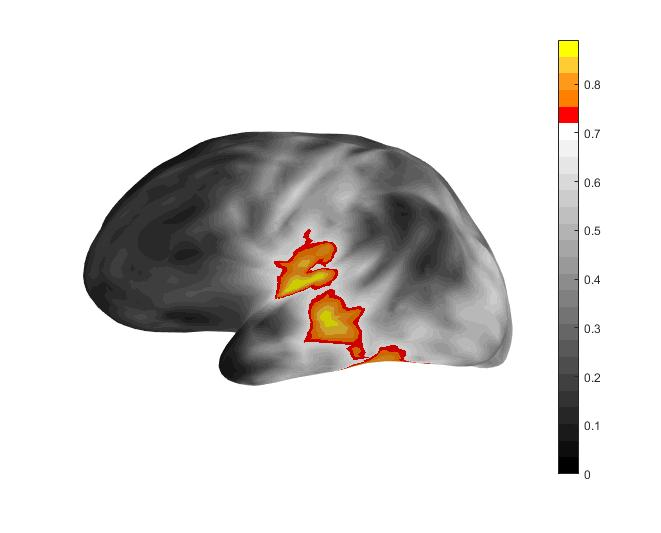
\includegraphics[width=0.7\textwidth]{kuulo.jpg}
    \caption{Kuva oikeiden aivojen mallilla vektori-MUSIC:lla. Kyseessä on kuuloärsykkeestä aiheutunut aktivaatio kuuloaivokuorella.}
\end{figure}

\begin{figure}
    \centering
    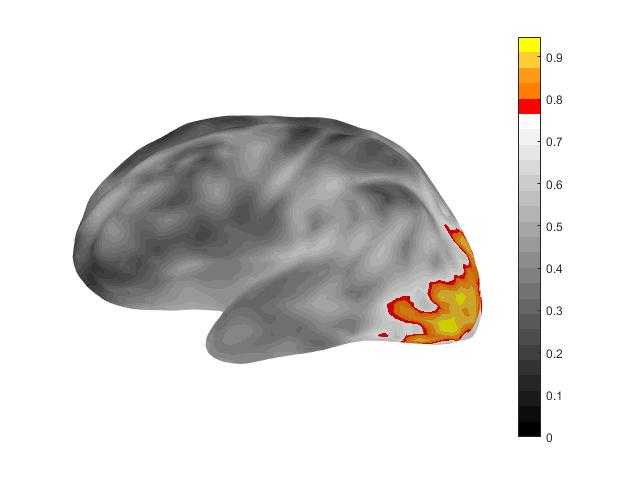
\includegraphics[width=0.7\textwidth]{esim1.jpg}
    \caption{Näköärsykkeestä aiheutunut aktivaatio havaittu näköaivokuorella.}
\end{figure}